\documentclass[15pt,landscape,twopage]{article}
\usepackage{amsmath,amssymb,amsfonts,amsthm}
\usepackage[english]{babel}
\usepackage[utf8]{inputenc}
\usepackage{fancyhdr}
%\usepackage[a3paper]{geometry}
\usepackage{geometry}
\usepackage{tikz}
\usepackage{xcolor}
\usepackage{float}
\usepackage{bm}
\usepackage{subcaption}
\usepackage{listings}
\usepackage{xcolor}
\usepackage{algorithm2e}
\usepackage{csquotes}
\usepackage{tikz}
\usetikzlibrary{automata,positioning}

\lstset{basicstyle=\ttfamily,
 showstringspaces=false,
 commentstyle=\color{gray},
 keywordstyle=\color{blue},
 morekeywords={grep, head, tail, cut },
 basicstyle=\footnotesize
}

\newcommand{\codepath}{../}
\newcommand{\gpath}{../plot}
\newcommand{\scriptpath}{../scripts}

\newcommand{\hr}{\begin{center} \line(1,0){450} \end{center}}
\newcommand{\R}{\mathbb R}
\newcommand{\B}{ \{0,1\} }
\newcommand{\tr}{^\mathsf{T}}
\newcommand{\F}{\mathcal{F}}
\newcommand{\norm}[1]{\left\lVert#1\right\rVert}
\DeclareMathOperator{\Id}{Id}
\DeclareMathOperator{\diag}{diag}
\DeclareMathOperator{\epi}{epi}
\DeclareMathOperator{\co}{co}
\DeclareMathOperator{\interior}{int}
\DeclareMathOperator{\Proj}{Pr}
\DeclareMathOperator*{\argmin}{argmin}
\DeclareMathOperator*{\argmax}{argmax}
\newcommand{\midd}{\mathrel{}\middle|\mathrel{}}


\newcommand{\generalPdfSymbol}{\bm{p}}
\newcommand{\gps}{\generalPdfSymbol}
\newcommand{\bernoulliPdfSymbol}{p_{bern}}
\newcommand{\binomialPdfSymbol}{p_{bin}}

\newcommand{\s}[1]{\sum_{#1}}
\newcommand{\am}[2]{\argmax\limits_{#1} #2}
\newcommand{\partition}[2]{\{ #1_1, #1_2, \dots, #1_{#2} \} }
\newcommand{\pd}[2]{#1 \left( #2 \right) }
\newcommand{\p}[1]{\pd{P}{#1}}
\newcommand{\cp}[3]{\pd{#1}{#2 \midd #3}}
\newcommand{\cpf}[3]{ \frac{\pd{#1}{#2,#3}} { \pd{#1}{#3} } }
\newcommand{\cpeq}[3]{\cp{#1}{#2}{#3} = \cpf{#1}{#2}{#3}}

\newcommand{\ltp}[3]{\s{#2_j \in \partition{#2}{n} } \cp{#1}{#3}{#2_j} \p{#2_j} }
\newcommand{\bysNom}[3]{\cp{#1}{#3}{#2_i} \pd{#1}{#2_i} }
\newcommand{\bys}[3]{ \frac{\bysNom{#1}{#2}{#3} }{ \ltp{#1}{#2}{#3} } }
\newcommand{\byseq}[3]{}


\newcommand{\bernoulli}[2]{ #1^{#2} \left(1 - #1\right)^{1 - #2}  }
\newcommand{\bern}{\bernoulli{\phi}{c}}

\newcommand{\likelihood}[1]{\prod\limits_{c \in C} #1 }


\geometry{top=20mm, left=20mm, right=10mm, bottom=15mm}

\pagestyle{fancy}
\lhead{Christian Lengert 153767}
\rhead{\today}
\chead{Graphical Models Lab : Latent Dirichlet Allocation (LDA)}
\rfoot{Page \thepage}

\begin{document}
\section{The model of Latent Dirichlet Allocation}
The model of Latent Dirichlet Allocation is a generative probabilistic model for collections of discrete data \cite{Blei2003}. Therefore it qualifies to be used for the explorative analysis of text corpora.
\subsection{Structure}

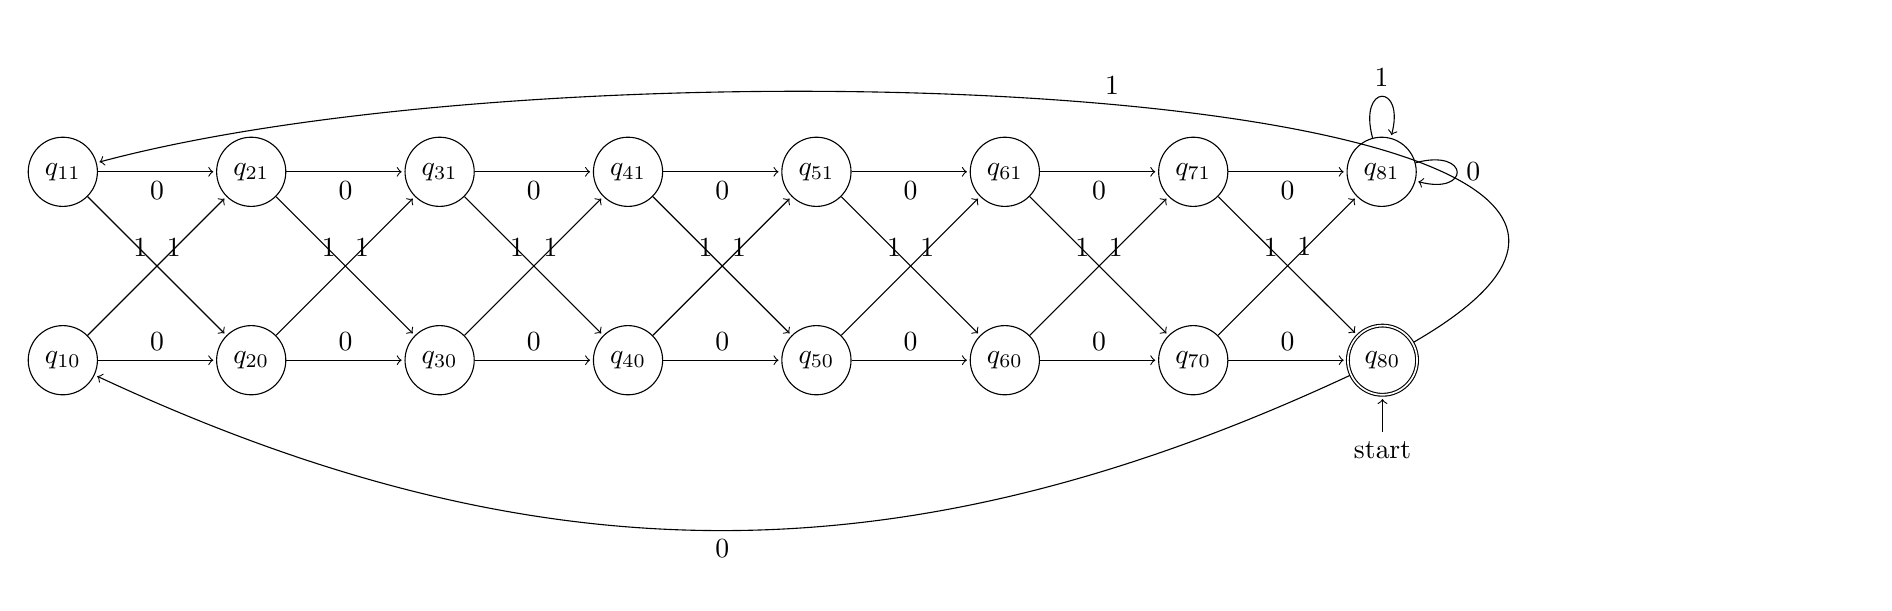
\begin{tikzpicture}[shorten >=1pt,node distance=1.5cm,auto]
 \node[state] (q_11)  {$q_{11}$};
 \node[state] (q_10) [below = of q_11] {$q_{10}$};
 
 \node[state] (q_21) [right= of q_11] {$q_{21}$};raving
 \node[state] (q_20) [right= of q_10] {$q_{20}$};
 
 \node[state] (q_31) [right= of q_21] {$q_{31}$};
 \node[state] (q_30) [right= of q_20] {$q_{30}$};
 
 \node[state] (q_41) [right= of q_31] {$q_{41}$};
 \node[state] (q_40) [right= of q_30] {$q_{40}$};
 
 \node[state] (q_51) [right= of q_41] {$q_{51}$};
 \node[state] (q_50) [right= of q_40] {$q_{50}$};
 
 \node[state] (q_61) [right= of q_51] {$q_{61}$};
 \node[state] (q_60) [right= of q_50] {$q_{60}$};
 
 \node[state] (q_71) [right= of q_61] {$q_{71}$};
 \node[state] (q_70) [right= of q_60] {$q_{70}$};
 
 \node[state] (q_81) [right= of q_71] {$q_{81}$};
 \node[state,accepting,initial below] (q_80) [right= of q_70] {$q_{80}$};
 \path[->]
 
 (q_11) edge  node {1} (q_20)
 edge  node [swap] {0} (q_21)
 (q_21) edge  node {1} (q_30)
 edge  node [swap] {0} (q_31)
 (q_31) edge  node {1} (q_40)
 edge  node [swap] {0} (q_41)
 (q_41) edge  node {1} (q_50)
 edge  node [swap] {0} (q_51)
 (q_51) edge  node {1} (q_60)
 edge  node [swap] {0} (q_61)
 (q_61) edge  node {1} (q_70)
 edge  node [swap] {0} (q_71)
 (q_71) edge  node {1} (q_80)
 edge  node [swap] {0} (q_81)
 
 (q_10) edge  node {1} (q_21)
 edge  node [above] {0} (q_20)
 (q_20) edge  node {1} (q_31)
 edge  node [above] {0} (q_30)
 (q_30) edge  node {1} (q_41)
 edge  node [above] {0} (q_40)
 (q_40) edge  node {1} (q_51)
 edge  node [above] {0} (q_50)
 (q_50) edge  node {1} (q_61)
 edge  node [above] {0} (q_60)
 (q_60) edge  node {1} (q_71)
 edge  node [above] {0} (q_70)
 (q_70) edge  node {1} (q_81)
 edge  node [above] {0} (q_80)
 
 (q_80) 	edge [out=30,in=15]  node [above] {1} (q_11)
 edge [bend left=25]  node [below] {0} (q_10)
 (q_81) 	edge [loop above]  node {1} (q_81)
 edge [loop right]  node {0} (q_81)
 ;
\end{tikzpicture}

\subsection{Variational Inference}


\section{Imlementation}
\subsection{Preparation}
First we have to choose a text corpus to estimate the parameters of the LDA-model from. For this we use a dump from the simple english wikipedia \cite{simplewi84:online}, namely the version named 'All pages, current versions only'.

For the purpose of speeding up the development process we will perform our operations on an even smaller subset of only 5 articles, to avoid long loading times on every run. We split some articles of the downloaded file into a smaller file with the script in section \ref{extract}.

\subsection{Class : Dataset}
We concentrate all operations regarding the preprocessing of the data in class named Dataset, which can be examined in section  \ref{class:dataset}. Our goal here is to process all articles and end up with a matrix of wordcounts, each row representing an article and each column representing a word. Therefore we have to establish a common dictionary containing all occurring words from all

\subsection{Class : LDA}

\section{Applying LDA}
\newpage

\bibliography{refs}
\bibliographystyle{IEEEtran}

\newpage

\section{Appendix}
\subsection{Extract subset} \label{extract}
\lstinputlisting[language=bash]{\scriptpath/extractSmallSubset.bash}

\subsection{Class : Dataset} \label{class:dataset}
\lstinputlisting[language=python]{\codepath/dataset.py}

\subsection{Class : LDA} \label{class:lda}
\lstinputlisting[language=python]{\codepath/inference.py}



\end{document}
